\documentclass[border=2pt,svgnames,tikz]{standalone}
\usepackage{fontspec}
\setmainfont{Source Serif 4}
\setsansfont{Source Sans 3}
\setmonofont{Source Code Pro}
\usetikzlibrary{arrows.meta, positioning, shapes.geometric, shapes.arrows, calc}

\begin{document}
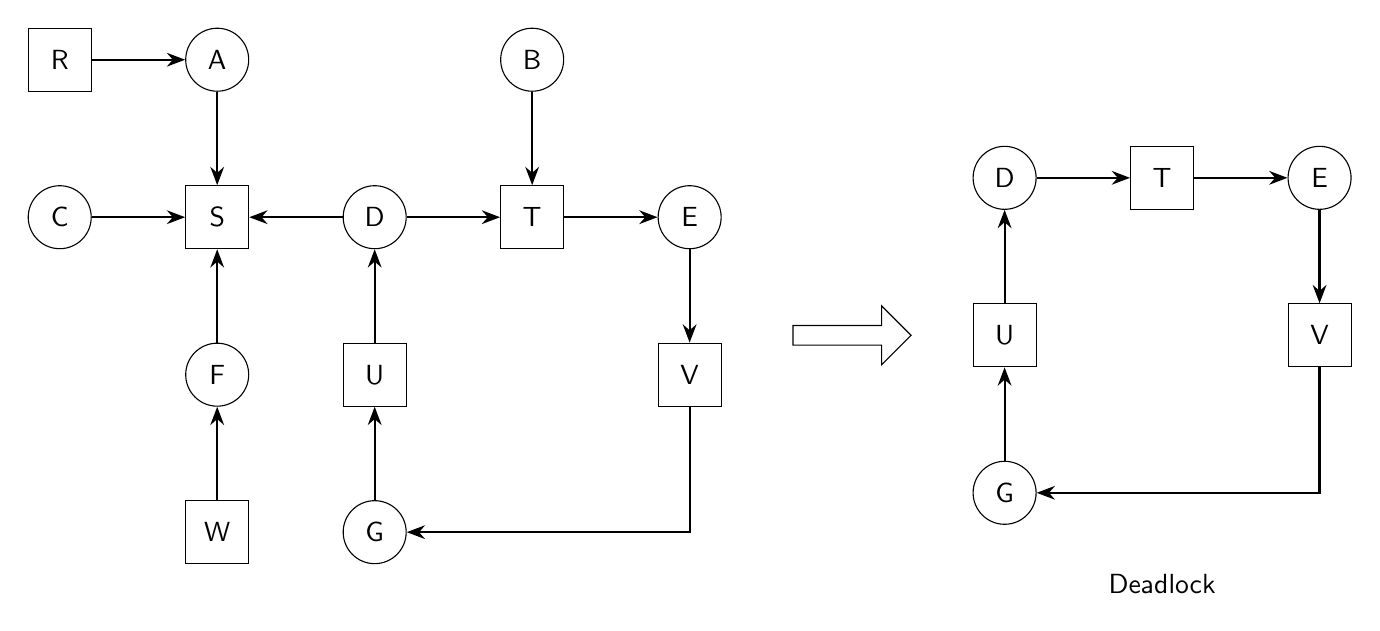
\begin{tikzpicture}[
    node distance=1.0cm and 1.0cm,
    resource/.style={draw, rectangle, minimum size=8mm, inner sep=2pt, font=\sffamily, fill=white},
    process/.style={draw, circle, minimum size=8mm, inner sep=2pt, font=\sffamily, fill=white},
    arrow/.style={-Stealth, thick},
    thick arrow/.style={single arrow, draw, fill=white, minimum height=1.5cm, shape border rotate=0}
]

% Left Graph
% Grid based placement
\node[resource] (R) at (0,0) {R};
\node[process] (A) at (2,0) {A};
\node[process] (B) at (6,0) {B};

\node[process] (C) at (0,-2) {C};
\node[resource] (S) at (2,-2) {S};
\node[process] (D) at (4,-2) {D};
\node[resource] (T) at (6,-2) {T};
\node[process] (E) at (8,-2) {E};

\node[process] (F) at (2,-4) {F};
\node[resource] (U) at (4,-4) {U};
\node[resource] (V) at (8,-4) {V};

\node[resource] (W) at (2,-6) {W};
\node[process] (G) at (4,-6) {G};

% Edges Left
\draw[arrow] (R) -- (A);
\draw[arrow] (A) -- (S);
\draw[arrow] (B) -- (T);
\draw[arrow] (C) -- (S);
\draw[arrow] (D) -- (S);
\draw[arrow] (D) -- (T);
\draw[arrow] (T) -- (E);
\draw[arrow] (E) -- (V);
\draw[arrow] (F) -- (S);
\draw[arrow] (W) -- (F);
\draw[arrow] (U) -- (D);
\draw[arrow] (G) -- (U);
\draw[arrow] (V) |- (G);

% Right Graph
\begin{scope}[xshift=12cm, yshift=-1.5cm]
    \node[process] (D2) at (0,0) {D};
    \node[resource] (T2) at (2,0) {T};
    \node[process] (E2) at (4,0) {E};

    \node[resource] (U2) at (0,-2) {U};
    \node[resource] (V2) at (4,-2) {V};

    \node[process] (G2) at (0,-4) {G};

    % Edges Right
    \draw[arrow] (D2) -- (T2);
    \draw[arrow] (T2) -- (E2);
    \draw[arrow] (E2) -- (V2);
    \draw[arrow] (U2) -- (D2);
    \draw[arrow] (G2) -- (U2);
    \draw[arrow] (V2) |- (G2);

    \node[font=\sffamily, below=0.5cm of G2, xshift=2cm] {Deadlock};
\end{scope}

% Big Arrow
\node[thick arrow] at (10,-3.5) {};

\end{tikzpicture}
\end{document}
